%!TEX root = main.tex
\section{Design of DawnPiper}
\label{sec:design}
\subsection{Design Overview}
The overall architecture of DawnPiper is illustrated in Figure~\ref{fig:sys_arch},
comprising three key modules responsible for pipeline parallelism partitioning.
Below, we provide a brief introduction to each module.
\begin{figure*}
  \centering
  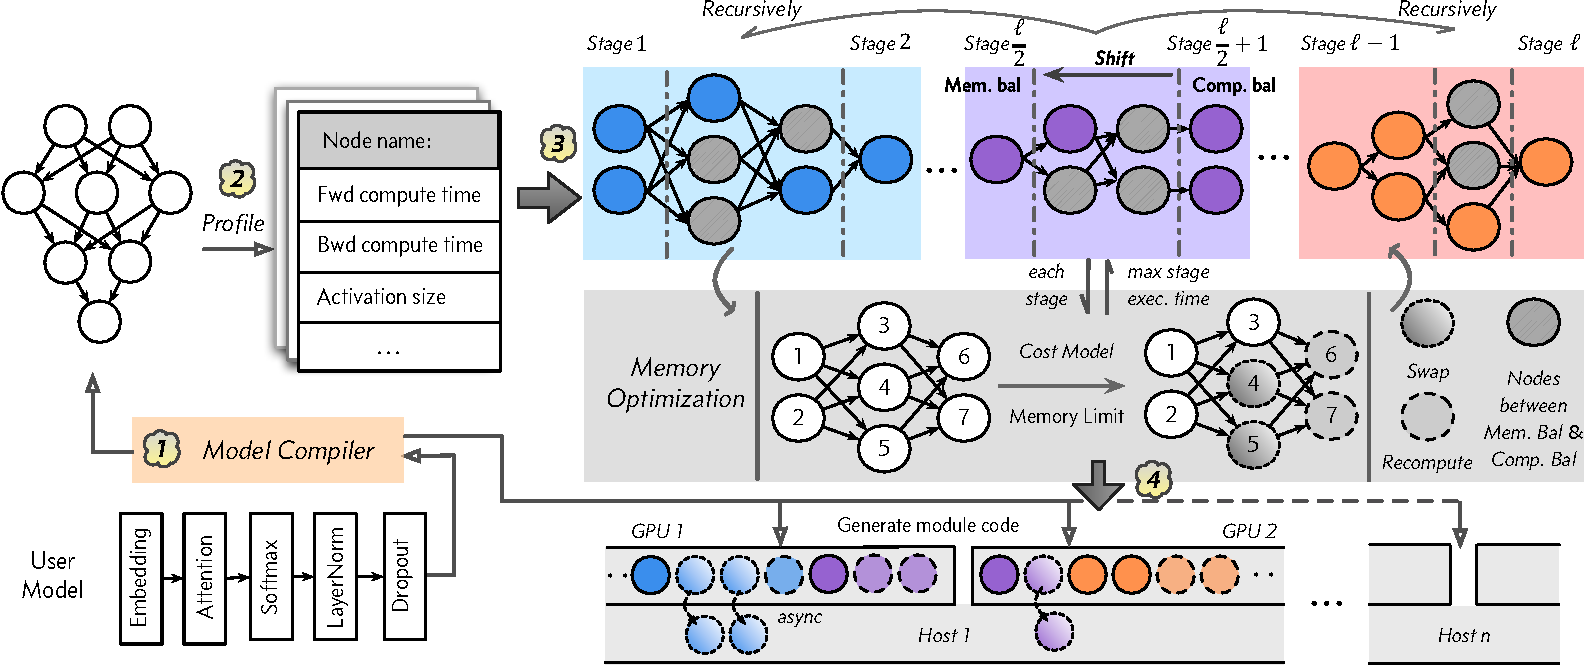
\includegraphics[width=0.95\linewidth]{pp-opt-arch-crop.pdf}
  \caption{DawnPiper System Architecture}
  \label{fig:sys_arch}
\end{figure*}

\textbf{Compiler:} When a model is submitted to DawnPiper,
the compiler generates a fine-grained computation graph using DL compilation techniques.
This graph captures all operators (nodes) involved in the training process along with their connections.
Leveraging this compilation-based approach enables precise model partitioning and memory optimization at a detailed level.
Additionally, the compiler automatically generates the code for each stage based on the partitioned sub-graphs,
removing the need for manual intervention and enhancing the system’s versatility and practicality.

\textbf{Profiling:} This module collects execution metadata for each node in the fine-grained computation graph.
For a node \emph{n}, the metadata includes forward computation time $t_f^n$,
backward computation time $t_b^n$, activation memory size $m_a^n$,
model parameters and optimizer states size $m_p^n$, and the list of saved tensors ${st}^n$.
The memory size that needs to be released at each node $m_d^n$ can also be inferred
via leveraging node dependency information.
With above data, the computation time, peak memory usage,
and inter-stage communication volume for any pipeline partitioning can be easily determined.
Additionally, this metadata informs memory optimization strategies.

\textbf{Pipeline Partitioning:} This module handles the pipeline partitioning process.
The key idea is to constrain partitioning within the range defined by the compute-balanced and memory-balanced points.
As each potential partition position is evaluated,
the memory optimization module identifies the minimum memory optimization cost
required to ensure each stage remains within GPU memory limits.
After evaluating all possible partition points,
the optimal strategy is the one where the longest stage has the shortest execution time.

In the following section, we will explore the pipeline partitioning and memory optimization algorithms in detail.

\subsection{Pipeline Terminology and Partition Theorem}
The number of pipeline stages is denoted $\ell$.
For a pipeline stage $x$, where $x \in [1, \ell]$,
the set of computation nodes it contains is represented as $\mathcal{N}_x$.
The computation time for this stage is determined by summing the
forward and backward computation times of all nodes in $\mathcal{N}_x$, as shown in Equation~(\ref{equ:tx}).
\begin{align}
  T_x=\sum_{n \in \mathcal{N}_x}\left(t_f^n+t_b^n\right)
\label{equ:tx}
\end{align}

The peak memory usage for a stage is calculated based on the nodes within the stage and the pipeline scheduling method.
The goal of optimal partitioning is to balance the computation times across all stages,
ensuring they are as close as possible.
Since inter-stage communication is minimal and can be overlapped with computation,
the objective is to minimize the execution time of the longest stage, i.e.,
the stage with the maximum computation time across all partitioning strategies.
This optimization is subject to the constraint that the peak GPU memory usage of
all stages remains within the GPU’s capacity.
In other words, the goal is to minimize $minimize\ \max_{1 \leq x \leq \ell} T_x$.

Given the fine-grained computation graph generated through DL compilation,
the search space for pipeline partitioning grows exponentially
when considering all possible partition points combined with different memory optimization strategies.
This makes the search space extremely large.
To address this, it is crucial to eliminate impractical partition strategies and reduce the overall search space.
We propose a partition theorem that leverages the memory usage characteristics discussed earlier
to effectively limit the partition space.

\textbf{Theorem:} For a model that needs to be divided into two pipeline stages,
the optimal partition point will lie within the closed interval between the
compute-balanced and memory-balanced positions, provided the following three conditions are met:
1) The computation time and memory usage during forward propagation exhibit
a monotonically increasing trend as operations are progressively scheduled;
2) The inter-stage communication time is consistently less than the computation time of each stage;
3) Memory optimization opportunities are evenly distributed across the model.

\textbf{Proof:} The compute-balanced and memory-balanced
partition points are denoted as $\rho_{cb}$ and $\rho_{mb}$, respectively.
In the 1F1B computation scheduling of asynchronous pipelines parallelism,
the earlier stages generally need to store more activation and parameter memory,
resulting in $\rho_{cb}$ typically being positioned further to the right than $\rho_{mb}$
(the reverse case can be proven similarly).
When the partition point is shifted to the right from $\rho_{cb}$,
more computation nodes are allocated to the first stage.
Due to the monotonic increase in both computation time and memory usage,
and given that inter-stage communication overhead is negligible,
the computation time and peak memory usage of the first stage increase,
while those of the second stage decrease.
Since memory optimization opportunities are evenly distributed across the model,
no stage with lower memory usage will require a disproportionately
high memory optimization cost to stay within the GPU memory limit.
Consequently, regardless of whether memory optimization is applied,
the first stage becomes the stage with the longest computation time,
surpassing the longest stage under the compute-balanced partition,
leading to a decline in pipeline training performance as the partition shifts rightward from $\rho_{cb}$.
Similarly, if the partition point is moved leftward from $\rho_{mb}$,
the second stage will become the one with the longest computation time
 which will continue to increase as the partition point shifts further left.

\subsection{Compute and Memory Balanced Partition}
In this section, we describe the process for determining the compute-balanced and memory-balanced partition points.
The general approach involves traversing the computation graph according to the execution order,
while continuously accumulating the forward/backward computation time or memory consumption.
Since asynchronous pipeline parallelism, such as in PipeDream,
requires accounting for stage-specific memory footprints
(due to differing numbers of activation and parameter copies across stages),
while computation time can be simply summed,
we focus on presenting the memory-balance partition algorithm for PipeDream, shown in Algorithm~\ref{alg:mem-ba}.

Before executing the algorithm, we first traverse the computation graph to determine the depth of each node.
Nodes with the same depth are then sorted based on the start time of forward computation,
forming the node set $\mathcal{N}_\mathcal{G}$, which serves as an input to the algorithm.
Additional inputs include the GPU peak memory limit $M_\mathcal{G}$ and the number of pipeline stages $\ell$.
The algorithm outputs the partition positions $\rho_x$ for each stage.
In PipeDream, the ratio of activation and parameter copies that need to be stored across stages is
$\ell:(\ell-1):(\ell-2):\cdots:1$.
If the peak memory usage of a micro-batch for each stage is denoted as $M_x$,
the following equation must hold to ensure balanced peak memory usage across all stages.
\begin{align}
  \ell \times M_1=\cdots=(\ell-x+1) \times M_x=\cdots=M_{\ell}
\end{align}
Based on this equation, the $M_x$ for each stage is computed,
as outlined in lines 2-5 and line 12 of Algorithm~\ref{alg:mem-ba}.
The algorithm then iteratively traverses the nodes,
first adding the activation memory, parameter memory,
and optimizer states memory of each node,
while checking if the accumulated memory exceeds the previously recorded peak memory.
Next, it subtracts the memory that needs to be released at the current node,
repeating this process until the accumulated peak memory reaches the target $M_x$ for the current stage.
At this point, the current node marks the partition point for that stage.
Although the description in the algorithm simplifies the partition point as a single node,
it typically involves a set of nodes in practice.
\begin{algorithm}
  \SetKwInOut{Input}{Input}
  \SetKwInOut{Output}{Output}
  $x \leftarrow 1,cur\_mem \leftarrow 0,peak\_mem \leftarrow 0$\;
  \For{$i$ in $[0,\ell)$}
  {
    $sum += \ell \div (\ell-i)$\;
  }
  $M_x \leftarrow M_\mathcal{G} \div sum$\;
  \For{$n$ in $N_\mathcal{G}$}
  {
    $cur\_mem += m_a^n + n_p^n$\;
    $peak\_mem \leftarrow \max(cur\_mem,peak\_mem)$\;
    $cur\_mem -= m_d^n$\;
    \If{$peak\_mem \ge M_x$}
    {
      $\rho_x \leftarrow n,x \leftarrow x + 1$\;
      $M_x \leftarrow (\ell \div (\ell -x + 1) \times M_1)$\;
      $cur\_mem, peak\_mem \leftarrow 0$\;
      \If{$x == \ell$}
      {
        \textbf{break}\;
      }
    }
  }
\caption{Memory balance partition in PipeDream}
\label{alg:mem-ba}
\end{algorithm}

\subsection{Binary Pipeline Parallel Partition}
If the peak memory usage of all stages under the compute-balanced partition is within the GPU memory capacity,
this partition strategy already represents the optimal pipeline partition in terms of performance.
However, if any stage exceeds the GPU memory limit,
the partition point must either be gradually adjusted from $\rho_{cb}$ toward $\rho_{mb}$
or memory optimization strategies must be applied to reduce memory usage.
Both methods alter the execution time of the stages,
making it difficult to predict which partition and memory optimization strategy will yield the best pipeline performance.
Consequently, a combinatorial search over these options is necessary.
In this process, for a given pipeline partition,
the goal of memory optimization for each stage is to minimize the optimization cost
while ensuring it stays within the GPU memory capacity.
Let $T_x^{moo}$ represent the minimum memory optimization cost time for stage $x$.
The objective then becomes $minimize\ \max_{1 \leq x \leq \ell} (T_x + T_x^{moo})$.

It is important to note that when shifting the partition point from $\rho_{cb}$ toward $\rho_{mb}$,
if the peak memory usage of the two adjacent stages after partitioning
are within the GPU memory capacity without requiring memory optimization,
further exploration of additional partition options is unnecessary.
This can be demonstrated by the theorem discussed earlier.
Briefly speaking, if the partition point continues to shift,
the computation time and memory usage of the stage with the higher computation load will keep increasing.
Whether memory optimization is needed or not,
the overall computation time for this stage will progressively rise,
surpassing the computation time of the longest stage at the current partition point.

Based on the above discussion,
a straightforward approach is to start from the compute-balanced partition $\rho_{cb}$ of
the first stage and iteratively move toward the memory-balanced
partition $\rho_{mb}$ while traversing possible partition points.
For each position, the $\rho_{cb}$ and $\rho_{mb}$ of the remaining $\ell - 1$ stages
are calculated until the last two adjacent stages are reached.
Memory optimization is then applied to determine the minimal cost for each stage.
Then we can record the computation time of the longest execution stage for the current partition position.
By traversing all partition possibilities, the optimal partition and memory optimization strategy can be identified.
Although the partition range is constrained between $\rho_{cb}$ and $\rho_{mb}$,
the search space grows exponentially with the number of pipeline stages.
To efficiently handle partitioning for deeper pipelines, we employ a binary partitioning approach.
This method first selects the middle stage of the pipeline,
treating the left and right segments as separate stages,
and applies compute-balanced and memory-balanced partitioning.
This approach allows the shortest computation time for the longest execution stage
on either side to be determined incrementally, level by level.
Once all possible partition positions have been explored at the outermost level,
the optimal partition strategy is identified.
This approach reduces the partitioning algorithm's complexity to $\mathcal{O}(\varphi^{log\ell})$,
where $\varphi$ represents the number of potential partition points traversed between $\rho_{cb}$ and $\rho_{mb}$.
This number is significantly smaller than the total number of nodes in the model.
For example, BERT has over 1000 nodes, but the number of nodes within this range is less than 100.
The overall process for this partitioning method is illustrated in Algorithm~\ref{alg:binary-partition}.
\begin{algorithm}
  \SetKwInOut{Input}{Input}
  \SetKwInOut{Output}{Output}
  \SetKwFunction{Fmain}{BinaryPartition}
  \SetKwFunction{Fadj}{AdjacentPartition}
  \SetKwProg{Fn}{Function}{:}{}
  \Fn{\Fadj{$\mathcal{N},sid$}}
  {
    $\rho_{cb},\rho_{mb} \leftarrow CompMemBalPartition(\mathcal{N}, sid, \ell)$\;
    \If{$\max_{sid \le x \le sid+1} ((\ell-x+1) \times M_x^{\rho_{cb}}) < M$}
    {
      \textbf{return} $\max_{sid \le x \le sid+1} T_x^{\rho_{cb}}$\;
    }
    $sorted\_pps \leftarrow IdentifyAndSort(\rho_{cb},\rho_{mb})$\;
    \For{$\rho \leftarrow sorted\_pps$}
    {
      $mopt_l,min\_t_l \leftarrow MemOpt(\mathcal{N}_{sid},M)$\;
      $mopt_r,min\_t_r \leftarrow MemOpt(\mathcal{N}_{sid+1},M)$\;
      $mopt \leftarrow mopt_l \cup mopt_r$\;
      $par\_dict[\rho] \leftarrow (\max(min\_t_l,min\_t_r),mopt)$\;
      \If{$!mopt$}
      {
        \textbf{break}\;
      }
    }
    \textbf{return} $\min(par\_dict)$
  }
  
  \Fn{\Fmain{$\mathcal{N},\mathcal{L},\mathcal{R}$}}
  {
    \If{$\mathcal{R}-\mathcal{L}==1$}
    {
      \textbf{return} $AdjacentPartition(\mathcal{N},\mathcal{L})$\;
    }
    $mid \leftarrow (\mathcal{L}+\mathcal{R}) /div 2$\;
    $\rho_{cb},\rho_{mb} \leftarrow CompMemBalPartition(\mathcal{N}, mid, \ell)$\;
    \For{$\rho \leftarrow sorted\_pps$}
    {
      $\rho_l,mopt_l,min\_t_l \leftarrow BinaryPartition(\mathcal{N}_{\mathcal{L}},\mathcal{L},mid)$\;
      $\rho_r,mopt_r,min\_t_r \leftarrow BinaryPartition(\mathcal{N}_{\mathcal{R}},mid+1,\mathcal{R})$\;
      $mopt \leftarrow mopt_l \cup mopt_r$\;
      $par\_dict[\rho] \leftarrow (\max(min\_t_l,min\_t_r),mopt)$\;
      \If{$!mopt$}
      {
        \textbf{break}\;
      }
    }
  }
\caption{Binary pipeline parallel partition}
\label{alg:binary-partition}
\end{algorithm}

The \texttt{AdjacentPartition} function in Algorithm~\ref{alg:binary-partition}
outlines the process for identifying the partition and memory optimization strategy
that minimizes the difference in computation time between two adjacent stages.
The compute-balanced $\rho_{cb}$ and memory-balanced $\rho_{mb}$ points
for these two stages can be derived by adjusting Algorithm~\ref{alg:mem-ba}.
Lines 7-8 describe the memory optimization procedure,
which determines the policy that results in the shortest execution time within the memory constraints.
Lines 10-13 allow for early termination of the traversal if no further memory optimization is needed between the two stages.
The function ultimately returns the optimal partition, memory optimization strategy,
and the corresponding execution time for the longer of the two stages.

The \texttt{BinaryPartition} function serves as the core of the binary partitioning algorithm.
Lines 18-19 call the \texttt{AdjacentPartition} function when only two adjacent stages remain.
Otherwise, the function calculates the compute-balanced and memory-balanced points when partitioning from the midpoint.
Lines 24-25 capture the optimal results for the left and right partitions,
which are recursively refined, including the partition points, memory optimization strategies
and the shortest execution time for the longest stage.
By invoking \texttt{BinaryPartition}$(\mathcal{N}_\mathcal{G}, 1, \ell)$,
the final optimal pipeline partitioning and memory optimization strategy is determined.

Note that while the algorithm assumes the number of pipeline stages to be a power of 2,
it is adaptable to any number of stages.
When the remaining stages are reduced to three,
the algorithm performs a traversal from the compute-balanced and memory-balanced partition positions of the first stage.
Therefore, the proposed approach is capable of handling any arbitrary number of pipeline stages.

\textbf{Communication Optimization:} A key assumption in the partitioning theorem is
that communication overhead should not impact the efficiency of pipeline parallelism.
Therefore, it is essential to avoid partition points that generate significant
communication volumes during the traversal within the partition range.
As discussed in Section~\ref{sec:mot}, the majority of computation nodes have very small activation memory.
First, we can identify inevitable communication points,
i.e., nodes with edges extending far outside
the partition range where data transmission is unavoidable regardless of the partition strategy,
such as the output of the initial embedding layer in BERT.
This inevitable communication can be disregarded.
For the remaining nodes, communication overhead can be minimized by optimizing the partition positions.
For instance, if activations from multiple nodes at the same depth need to be transmitted to the next stage,
the algorithm can identify the lowest common leaf node connecting these edges.
If this leaf node is the sole connection point,
the partition can be adjusted so that only the activation of this single node is transmitted, instead of multiple nodes.
Such leaf nodes are typically easy to locate,
resulting in minimal impact on both the computation time and memory usage of the adjacent stages.

\subsection{Memory Optimization}
The goal of memory optimization is to minimize the execution time of each stage
while adhering to the GPU memory limits for a given partitioning.
This objective is very similar to memory optimization in single-GPU training.
To achieve this, we employ the cost model from Capuchin~\cite{pengCapuchinTensorbasedGPU2020},
which evaluates memory swapping and recomputation using \emph{FreeTime} and \emph{Memory Saving Per Second (MSPS)}.
The model first applies memory swapping until data transfer can no longer overlap with computation.
Then, it selects the method either memory swapping or recomputation that incurs the smallest performance overhead.
In DawnPiper, memory optimization candidates are easily identified through each node's saved tensors list,
and their \emph{FreeTime} and \emph{MSPS} can be calculated from the node’s metadata.

However, there are specific considerations for memory swapping in pipeline parallelism.
Typically, multiple GPUs share the same host memory, which imposes limits on CPU memory availability.
For instance, an 8-GPU A100 server that requires 40 GB of memory swap per stage
would need a total of 320 GB of CPU memory.
Additionally, this CPU memory must be page-locked to maintain the asynchrony of memory swapping,
further constraining this resource.
Consequently, we limit the memory swapping size to one-fourth of the total host memory size based on practical experience.
Another consideration is that in a 1F1B scheduling pipeline parallelism,
a single memory swap operation within a micro-batch can result in multiple swaps of the same memory.

% Although the interval between memory swapping out and swapping in in the earlier stages is not only the inter-layer computation
% in single-GPU training but also the computation of different micro-batches, for inputs with the same micro-batch number,
% its memory swapping in cannot be performed before the start of its backward computation,
% as this would cause a memory shortage in the forward computation of other micro-batches.
% This means that the computation time available for overlapping data transfer in memory swapping is consistent
% in pipeline parallel training and single-GPU training.
% The assessment of recomputation benefits is unified in these two training modes, that is,
% to exchange less recomputation time for greater memory occupation reduction.
% Therefore, this section uses the memory optimization method in single-GPU training to
% find the minimum cost memory optimization strategy for each stage in pipeline parallelism that meets the memory limit.
% This method only needs to traverse the nodes once, as shown in Algorithm 3.3.
% First, line 1 calculates the amount of memory that needs to be saved for the current stage $x$.
% Secondly, recomputation uses the amount of memory that can be saved per second in single-GPU memory optimization
% to assess the benefits of recomputation for each node, that is, for each node after model compilation,
% calculate their ${MSPS}_n = \frac{m_a^n}{t_f^n}$, the larger the MSPS means the greater the recomputation benefit.
% Memory swapping uses the memory swapping idle time to assess its benefits.
% In this way, through the list of tensors saved for each node in the model test and analysis,
% all node output activation values that need to be saved during the backward computation process can be obtained,
% and then they can be sorted according to the above benefit estimation formula, as shown in line 2.
% Then, for each candidate memory optimization object, calculate their memory optimization cost and recomputation cost.
% If the current memory size of memory swapping has exceeded the preset threshold, then recomputation will be performed at this time.
% When the total amount of memory for memory optimization reaches the amount of memory that needs to be saved, exit,
% so as to obtain the strategy of minimum memory optimization cost under the memory limit.
